% vim: foldmethod=marker foldcolumn=3

% {{{ 选题
\chapter{选题依据及意义}

数据中心被目前的企业中所广泛采用,
大型的数据中心甚至承载着公司的服务系统. 其中
服务器与服务器之间几乎完全是通过现代网络所连接.
用户对网络性能的要求日益扩大, 一些微小故障, 很可能会造成用户体验的下降,
特别是在某些交互敏感的场合. 服务的质量必须得到保证. 可是对于庞大的系统,
各种问题的发生是无法避免的. 我们只能更快, 更精准的解决问题,
以此将故障的危害降到最低. 这也是对新时代的检测调试 工具的挑战.

面对大型复杂数据中心的调试以及错误, 如果仍然使用简陋的单机调试手段,
例如\texttt{ping}, \texttt{tracerout}, 也许可以解决问题, 但其代价与耗时,
是无法满足运营要求的. 进而, 许多公司提出了自己的方案,
甚至为自己搭建的集群开发出一套相匹配的网络调试工具.



\chapter{研究目标和主要内容(含论文提纲)}

在数据中心网络(DCN)中, 众多网络设备运行过程中的故障在所难免,
及时发现故障并确定 故障位置成为DCN网络运维的重要组成部分.
本课题参照微软提出的Everflow故障检测方案,
设计实现一款面向数据中心网络的流量分析与故障检测工具.

为了解决现实存在的数据中心的网络异常问题, 利用现有交换机的\textbf{Match and Mirror}
机制, 将特定的数据包进行镜像. 分析镜像后的数据包, 以达到对网络中存在问题的检测.

本次设计中, 将会基于通用的处理器平台, 关注于DCN中环路的检测, 结果保存,
预警, 数据展示, 探针构造几个方面. 初步实现Everflow功能的基础上,
进行了简单的改进完善, 以下列出了程序的主要功能:

\begin{itemize}
\item
  对实时采集到的数据包进行分析,
  实现丢包检测,环路分析或时延异常等故障检测;
\item
  加入了对快慢路径两种不同的分析方案;
\item
  在分析时, 多处使用hash数据结构来加快查找, 以加快处理速度;
\item
  按需保存Trace数据并在必要时生成主动探测包,
  以进一步确定故障位置和故障原因;
\item
  采用B/S架构, 管理员通过浏览器即可进行操作
\end{itemize}

% }}}

% {{{ Everflow简介
\chapter{Everflow简介}

  Everflow \cite{greenberg2016packet} 这是微软在2015年发表的论文. 与部署
运行超过了4年的Pingmesh \cite{guo2015pingmesh}不同, 它并没有特别关注
端对端的延迟, 而是从数据包层面进行分析.

  对于Everflow来说, 最大的挑战莫过于扩展性了. 大型DCN(10W以上的服务器)中流量
轻松就能达到100Tbps, 追踪这样规模的数据包需要大量的网络资源与服务器资源,
想象一种典型的情况, 平均每个包的大小为1000bytes,
每个镜像数据包64bytes(只包括头部信息), 并且网络的直径为5跳. 如果我们
简单的追踪每个数据包的每一跳作为数据包历史, 数据流量就会有这么多
$\frac{64B}{1000B} \times 5(hops) \times 1000(Tbps) = 32(Tbps)$, 如此高的追踪流量
将会造成网络拥塞和丢包, 特别是当网络利用率很高时.

  另一个扩展性的挑战是路径分析. 因为商用交换机有限的存储与CPU运算能力, 追踪数据包
必须由服务器来完成. 即使假设一个服务可以处理10Gbps的流量, 我们需要
$\frac{32Tbps}{10Gbps} = 3200$这么多服务器来处理, 这也是很大的开销.


\begin{figure}
  \centering
  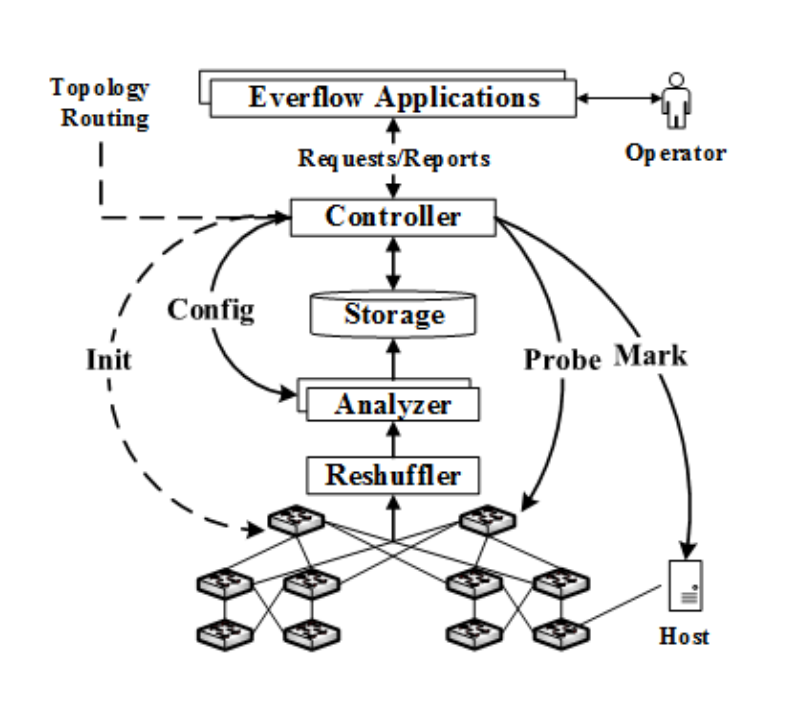
\includegraphics[width=0.8\textwidth]{../img/everflow_arch.png}
  \caption{Everflow的路径收集与分析流水线}
  \label{fig:everflow_arch}
\end{figure}

  如图\ref{fig:everflow_arch}所示为Everflow的架构.

  Everflow的关键思想在于镜像特定的报文, 在商用交换机上设置特定的匹配规则, 匹配后执行
相应的动作(将数据包发出). 另外利用交换机内置的ASIC芯片的负载均衡, 将捕获到的包
重新分发到不同的分析服务器上, 另外它也能发送定向探针去确认潜在的错误.

  它由四个主要组件组成: 控制器, 分析器, 存储器以及洗牌器. 在顶层, 有许多应用程序使用由
Everflow提供的信息去调试网络错误. 控制器负责协调其它组件以及和应用程序交流. 在
初始化过程中, 它配置交换机上的规则. 被匹配到的数据包将会镜像至洗牌器中, 而后会直接
到达分析器中, 而后将分析结果传递至存储器中. 控制器也提供了一些API, 允许Everflow
的应用程序去查询分析结果, 并且在主机上设置debug位.

  2014年, 微软工作人员在微软两个的数据中心上进行Everflow部署.
第一个部署的是前期制作的集群,其中有37台交换机. 第二个部署是对生产环境的
2500台交换机中的440台进行部署. 两个集群承载了许多应用程序的流量.
除此之外, 工作人员也在特定的生产交换机上开启了Everflow, 用以支持在线错误的调试.
目前, 微软工作人员也扩展了Everflow的部署以使其可以被更多的交换机和集群使用.
通过部署在微软的DCN上, Everflow证明了其作为诊断DCN错误不可或缺的工具的实用性.
% }}} Everflow简介

% {{{ 功能概述
\chapter{功能概述}

本次的设计分为三大部分. 分析器, 控制器, 以展示页面, 以下分别进行概述,
更加详细的 实现细节请查看实现方案\ref{chap:实现方案}.

\begin{figure}
  \centering
  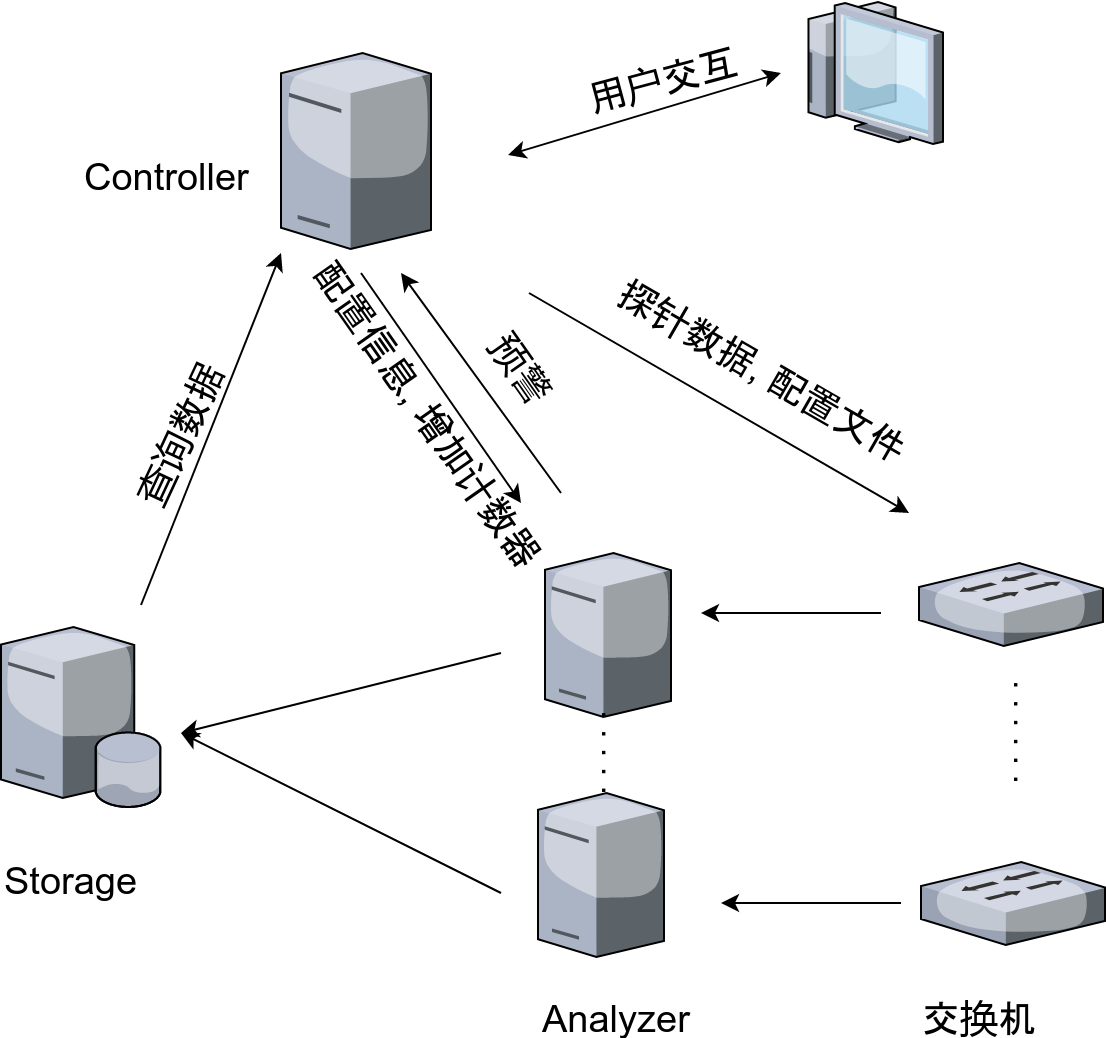
\includegraphics[width=0.7\textwidth]{../img/user_flow.png}
  \caption{architecture}
  \label{fig:arch}
\end{figure}

图\ref{fig:arch}中介绍了整个系统的结构.

\section{分析器功能概述}

  分析器是一群分布式的服务器, 且每个服务器处理一部分的追踪流量.
  分析器读入产生的数据包后, 进行初步的处理, 而后存入存储器中供控制器使用.
在分析器中, 我们可以获得整条的数据包路径, 通过路径,
我们可以得知是否有环, 或是有丢包现象. 以及对于特定的模式进行统计,
对于探针来说也可以粗略的衡量延迟.

分析结束后, 并不是所有的结果都要存入存储器, 只有异常行为数据流,
有debug标志的数据流, 重要协议(BGP, PFC等)会被记录到存储器中.

\section{存储器功能概述}

存储器中, 主要存储分析器产生的结果, 包括网络流数据与相应规则的统计数据.
使用MySQL进行数据存储, 具体的表格见\ref{chap:数据库设计}.

  网络流数据表格中, 每一行对应给一个追踪记录. 包括数据包的每一跳信息, 以及
数据包的元信息, 是否为探针, 是否有环, 是否丢包, 它们可以在查询时指定规则
来进行过滤.

  我们也在表格中存储了所有分析器产生的计数器, 表中的每一行代表着从分析器取得的
计数器的ID以及, 记录时间, 分析器ID.

  同时, 存储器中, 也存储了全部的统计规则.


\section{控制器功能概述}

控制器最重要的功能就是向外提供API接口. 除此之外, 控制器可以对分析器配置,
向交换机中发送探针, 分析器对于探针会单独提供支持.
目前我们能够提供的API包括 按时间查找数据流, 查询计数器的值, 添加探针,
以及发生错误后的预警功能.


\section{访问页面功能概述}

此部分主要展示存储器中的数据, 包括网络流数据, 不同的规则下的统计数据;
以及提供用户与程序的交互能力, 包括增加删除统计规则, 探针的构造及发送.

% }}}功能概述

% {{{ 实现方案
\chapter{实现方案}
\label{chap:实现方案}

\section{分析器}

下图\ref{fig:analyzer_process}是具体处理过程. 首先进行
对GRE数据包的解封操作, 解封后, 使用多线程并发分析. 解封后,
具有相同标示的数据包 需要进入相同的线程中.

分析中, 如果某一跳交换机在1s内, 没有收到接下来的报文,
即认为此次数据包已经结束, 因此, 我们需要增加定时功能.
相关算法请查看主要算法说明\ref{chap:主要算法说明}中定时器的实现.

\begin{figure}
  \centering
  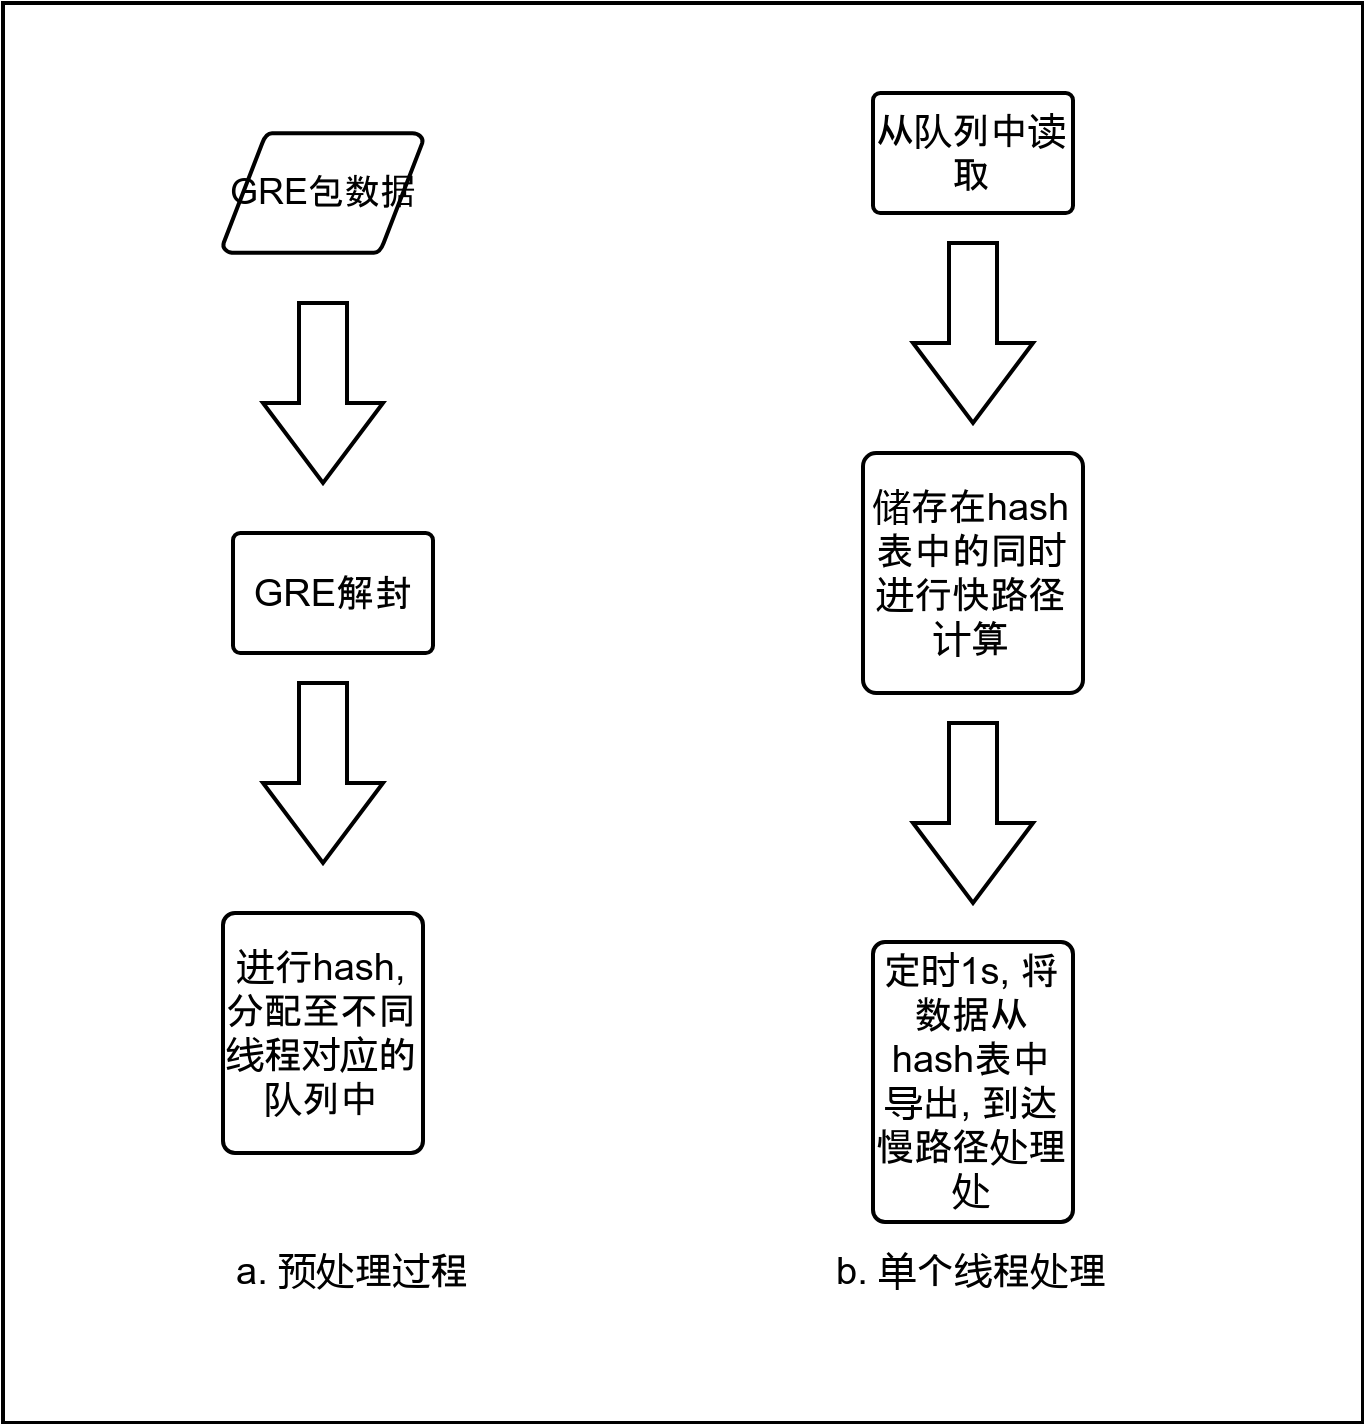
\includegraphics[width=0.9\textwidth]{../img/analyze_process.png}
  \caption{Analyezr process}
  \label{fig:analyzer_process}
\end{figure}

上述的流程图可能并不直观, 以下\ref{fig:analyzer_arch}为程序实际的处理流程,
其中的英文关键字为程序中确切的类名. 其中,
Reader与Processer均可以自行配置个数.

\begin{figure}
  \centering
  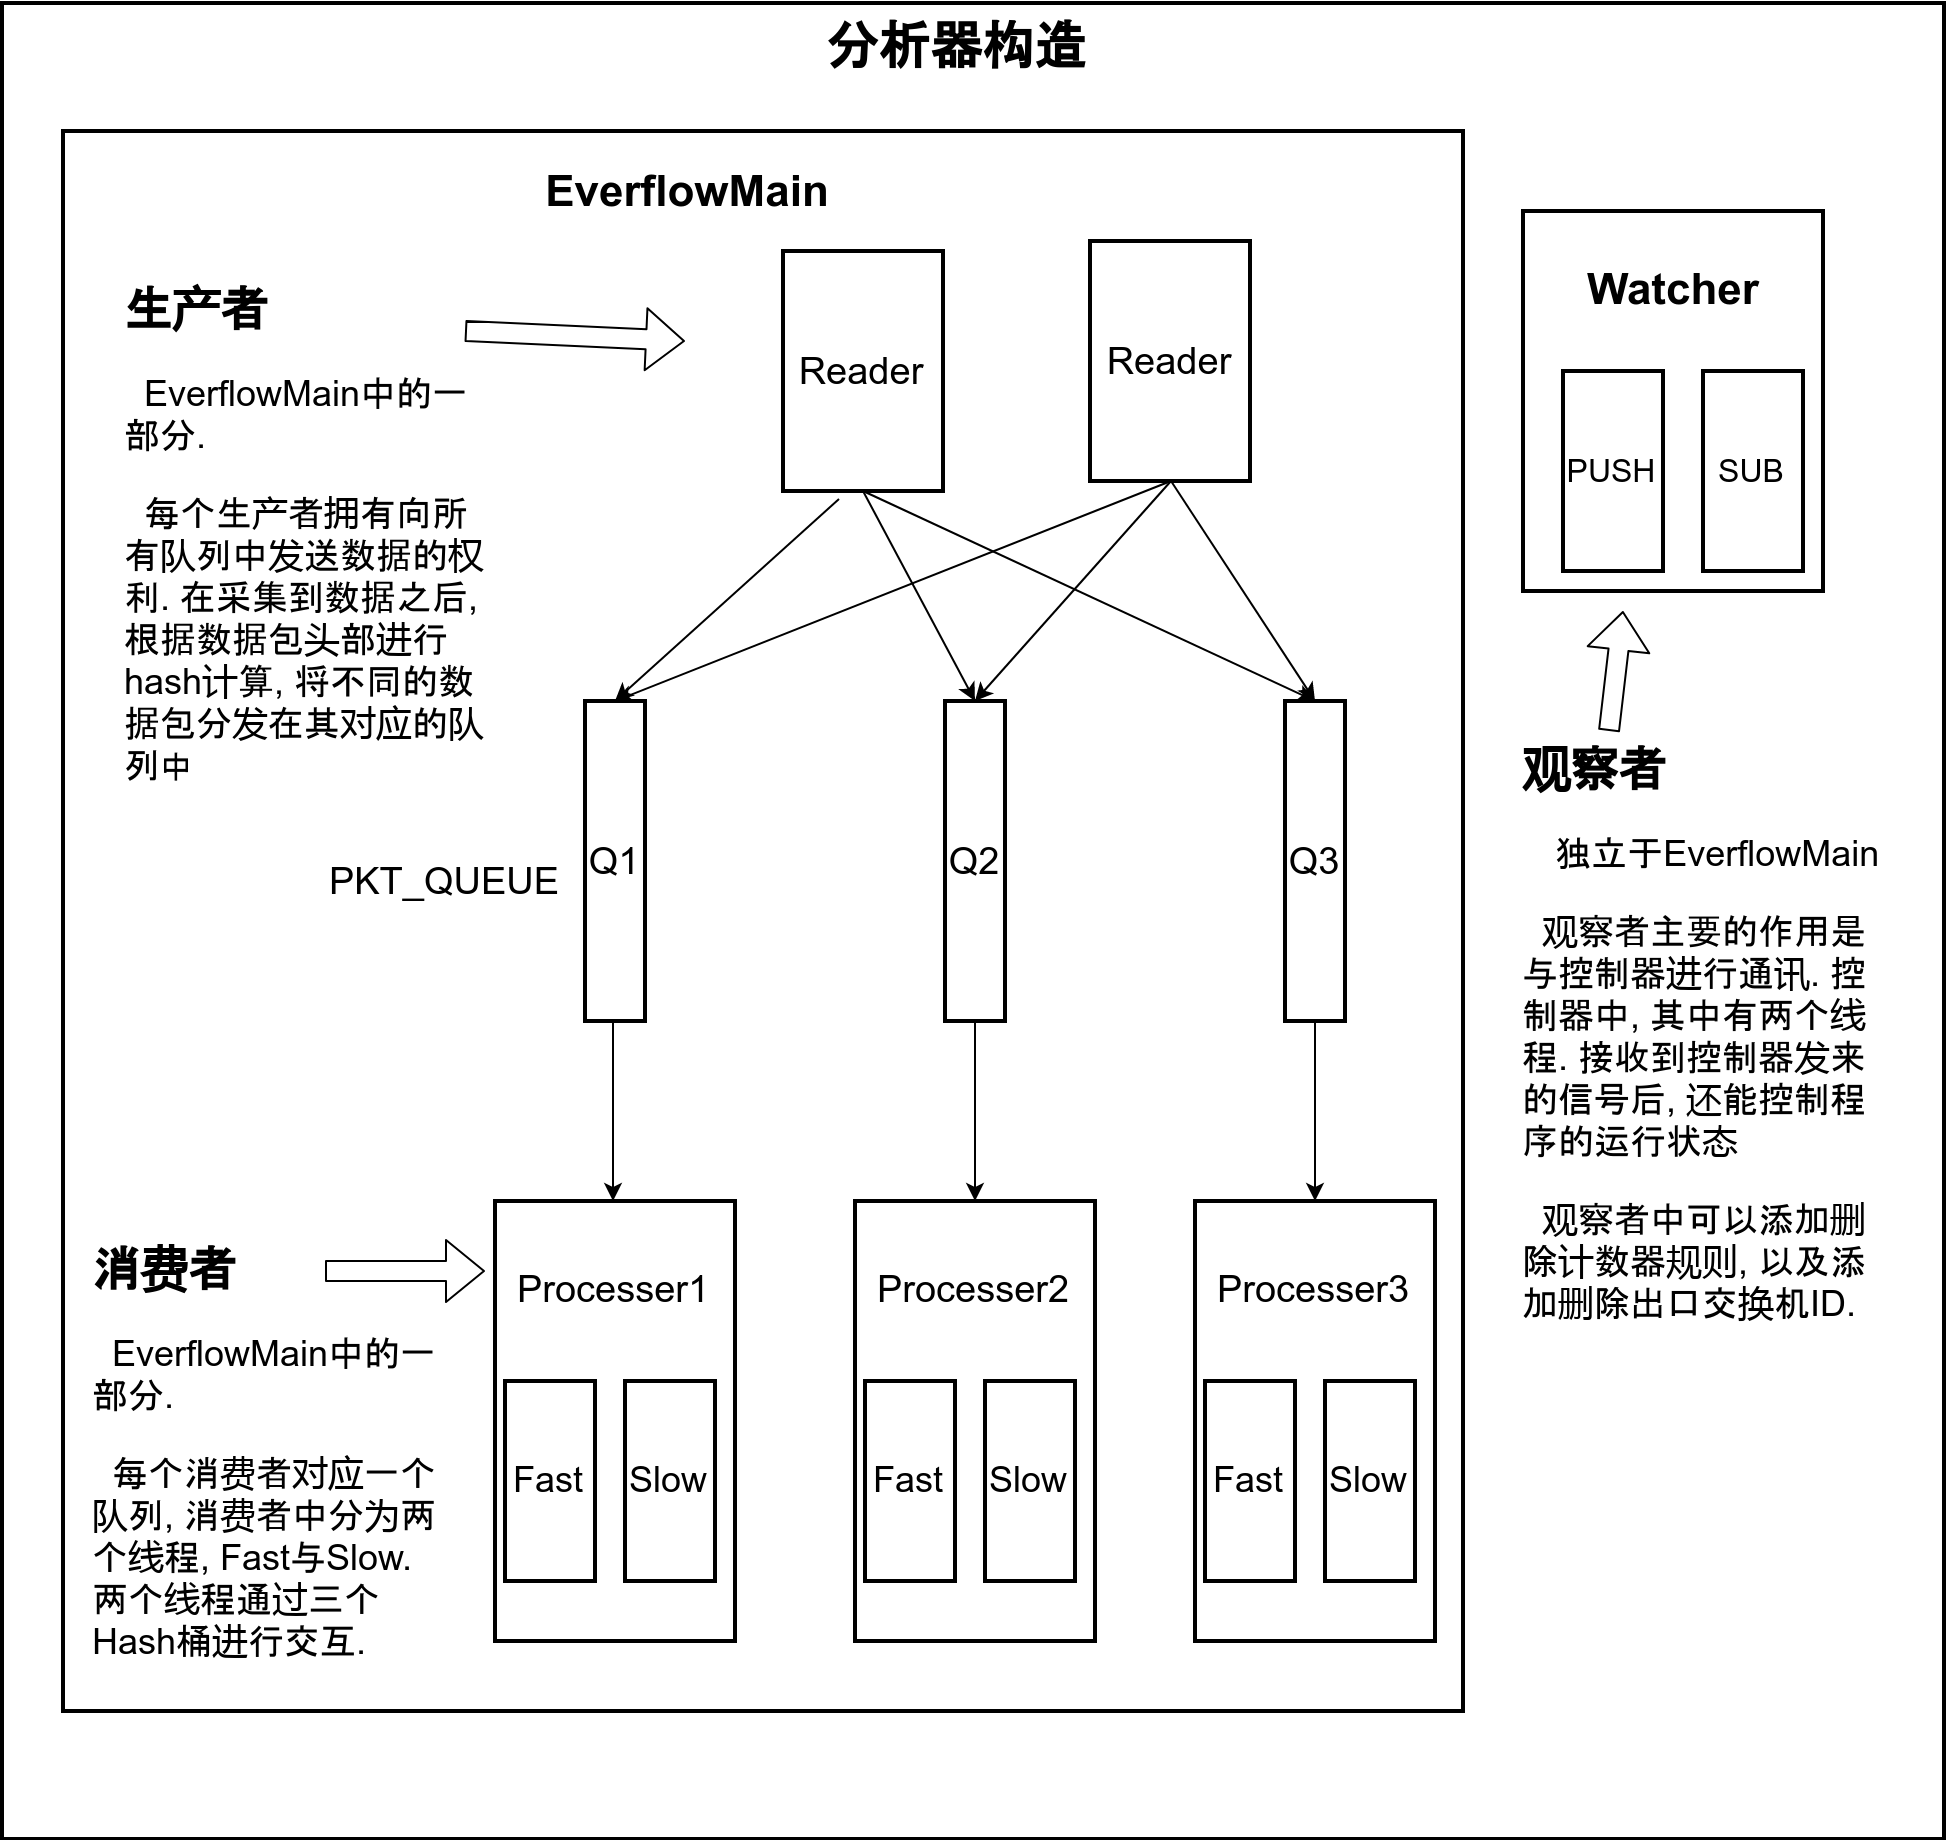
\includegraphics[width=0.9\textwidth]{../img/analyzer_structure.png}
  \caption{Analyezr Architecture}
  \label{fig:analyzer_arch}
\end{figure}

\subsection{程序启动流程}

启动时, 首先初始化\texttt{Watcher}, 继而向控制器发送\texttt{INIT}信息,
请求出口交换机信息 与最新的统计规则. 收到控制器的回复后,
启动\texttt{Processer}, 而后启动\texttt{Reader}, 这
时的\texttt{Reader}开始获取\texttt{GRE}数据包, 并根据内层的五元组(源IP,
目的IP, 源端口, 目的端口 协议类型)进行hash操作,
按照不同的结果存入到相应的队列中, 供\texttt{Processer}使用.

\subsection{程序退出流程}

程序停止时, \texttt{Watcher}首先向控制器发送\texttt{QUIT}信号,
通知控制器, 当前的分析器准备 停止了, 而后, 控制器做出回应.
每个控制器下监管许多分析器, 他有权也应当知道所有分析器的 状态.

程序中多次使用了队列进行解耦, 如果队列为空, 那么所有的消费者将会被阻塞.
程序 收到退出信号时, 一定是先将生产者全部停止, 待生产者全部停止后.
依次向队列中发送截止数据包, 向消费者表明生产者已经不再继续生产了.
可以停下来了.

\subsection{分析器实现中遇到的问题及解决方案}

分析器是本次设计的核心, 分析器遇到的问题是最多的, 篇幅很大,
这里只列出问题的名称. 在程序中的问题及解决\ref{chap:程序中的问题及解决}中详细列出.

\begin{itemize}
  \item 毫秒级时间戳的使用
  \item 与控制器的交互问题
  \item Counter计数器表格的设计问题
  \item 程序中内存泄露问题
  \item 定时器与signal
  \item 分析器的启动过程
  \item 与控制器的交互问题
  \item 热重启与容灾问题
\end{itemize}
\section{控制器}

控制器采用\texttt{Python}实现. 使用了\texttt{Tornado}进行实现. 它向下控制分析器
向上为应用程序提供接口. (技术选型请查看设计中的一些抉择
\ref{chap:设计中的一些抉择})


\begin{figure}[htbp!]
  \centering
  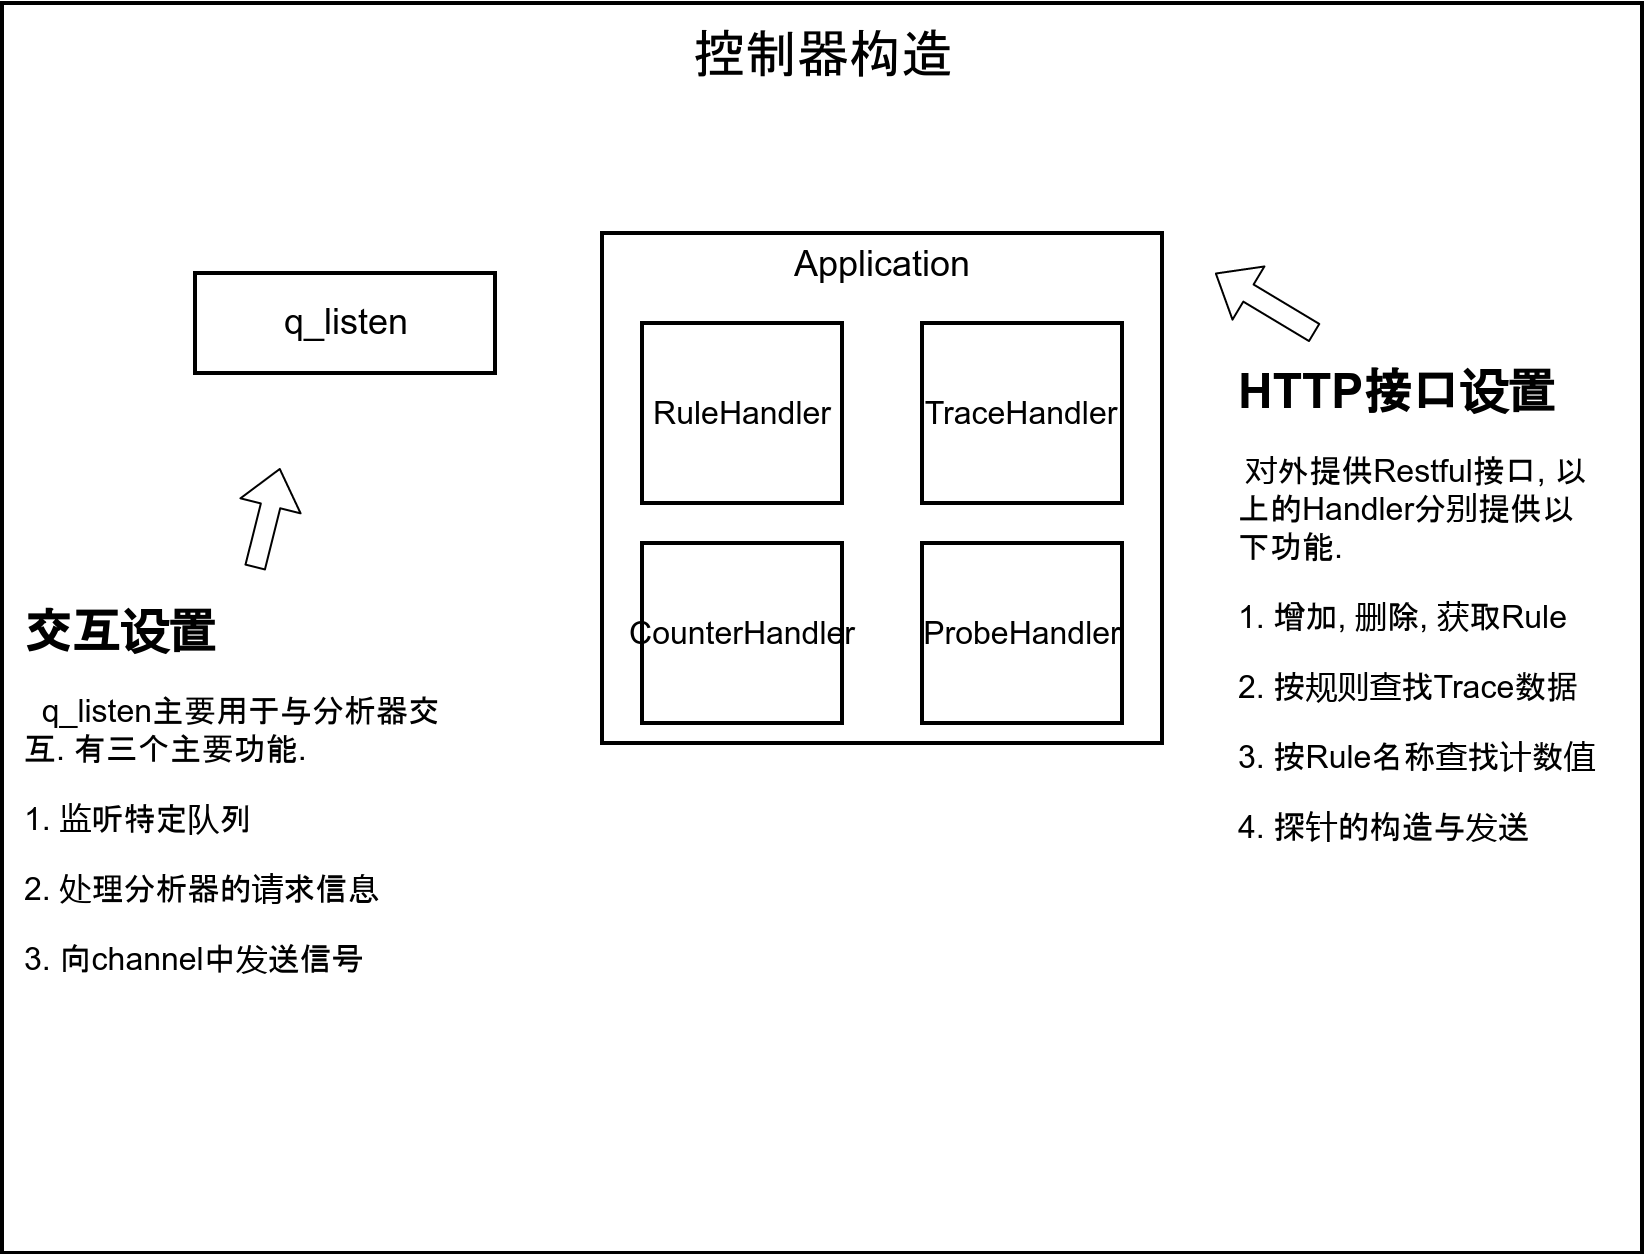
\includegraphics[width=0.9\textwidth]{../img/controler_arch.png}
  \caption{Controler Architecture}
  \label{fig:contoler_arch}
\end{figure}

控制器中, 涉及到两个方面:
一是与存储器的交互, 这里, 我们的存储器使用\texttt{MySQL};
二是与分析器进行交互, 通过\texttt{Redis}进行解耦.


\textbf{与存储器交互}: 允许用户读取Trace记录, 读取统计信息. 允许用户读写统计规则,
以及构造探针

\textbf{与分析器交互}: 每个分析器启动时, 需要首先向控制器发送请求, 获得控制器的
允许后, 才能启动. 并且, 如果用户更新了统计规则, 控制器也会立刻下发到所有的的
分析器中. 在分析器准备结束时, 也同样需要请求控制器. 未来的控制器可能还需要添加
对于每个分析器的管理功能.


\section{访问页面}

下图\ref{fig:traffic_data_show}, \ref{fig:counter_data_show}


% 分别展示了数据流量的显示以及 计数器结果的显示, 目前主要列出信息模块,
% 搜索功能会接着完善.

\begin{figure}[htbp!]
  \centering
  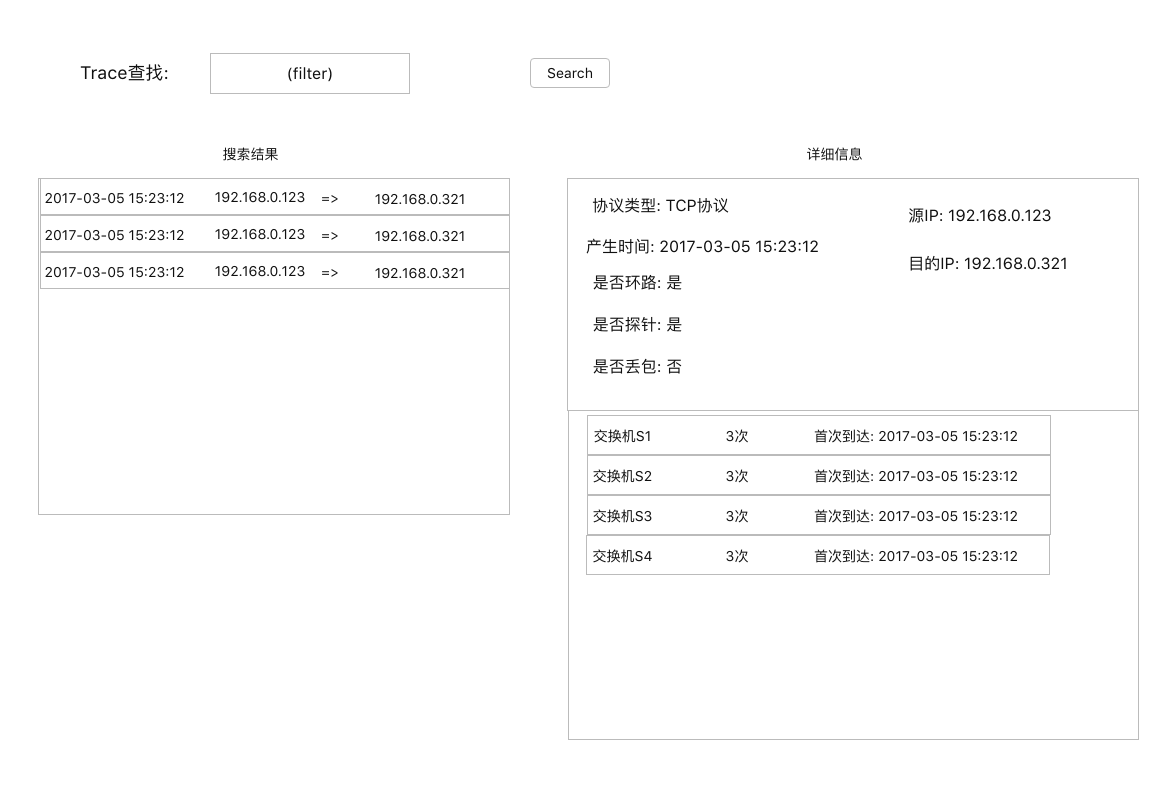
\includegraphics[width=0.9\textwidth]{../img/traffic_data_show.png}
  \caption{Traffic data}
  \label{fig:traffic_data_show}
\end{figure}

\begin{figure}[htbp!]
  \centering
  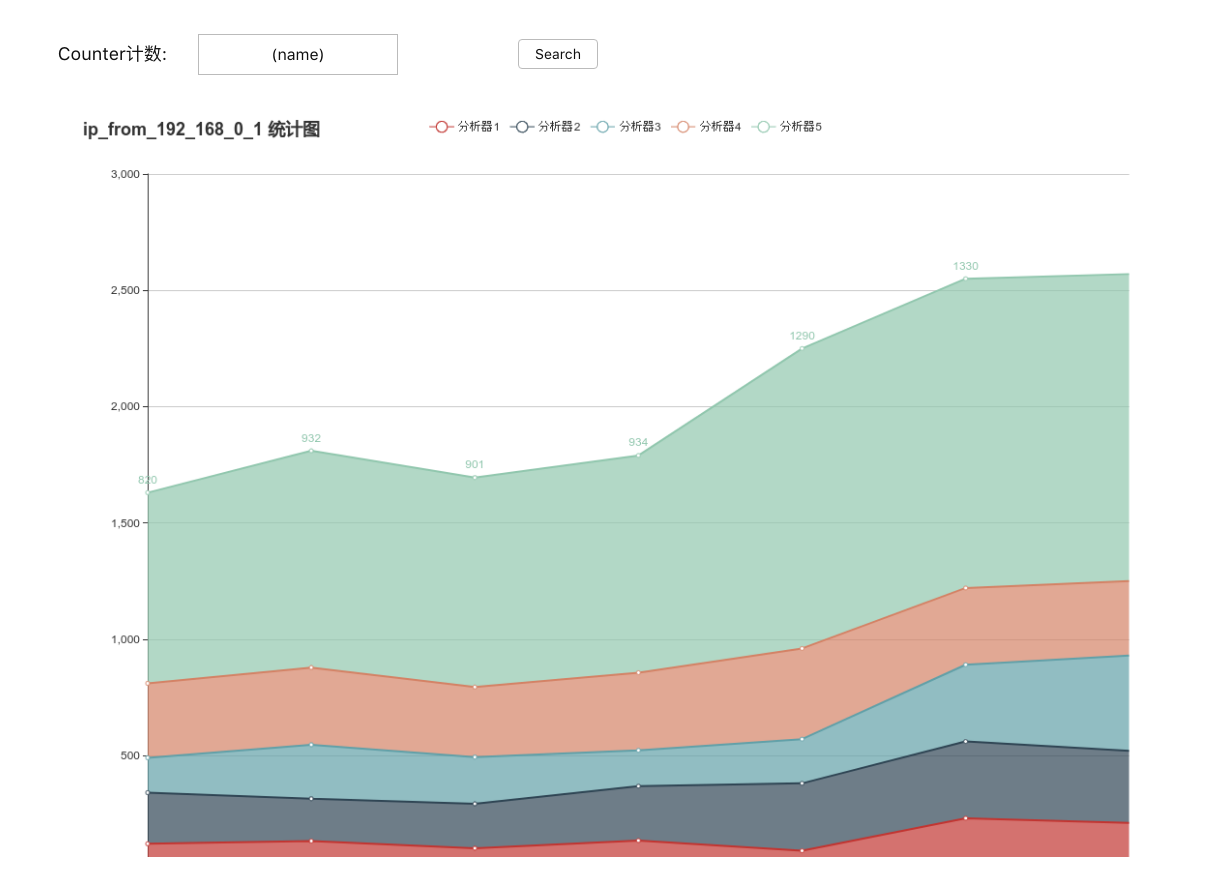
\includegraphics[width=0.9\textwidth]{../img/counter_data_show.png}
  \caption{Counter data}
  \label{fig:counter_data_show}
\end{figure}

% }}} 实现方案

% {{{ 接口设计
\chapter{接口设计}\label{chap:接口设计}

\section{分析器, 控制器接口设计}
\label{sec:分析器, 控制器接口设计}

\subsection{启动过程}

每台分析器启动时, 首先向控制器发送请求. 获取计数器规则, 以及出口交换机ID,
这里是向控制器监听的队列中发送.

\begin{lstlisting}
{
  "ACTION": "INIT",
  "ANALYZER_ID": 124         // 分析器ID, 由分析器的配置文件进行配置
}
\end{lstlisting}

控制器收到报文后, 寻找可用的ID, 进行返回, 同时带上出口交换机的ID, 以及计数器信息
通过控制器进行配置, 可以简化分析器的操作.

\begin{lstlisting}
{
  "ANALYZER_ID": 124,           // ID为0, 表示这是一种广播操作.
  "MESSAGE": {                  // 报文主体
    "COMMOND": "INIT",          // 初始化
    "SWH_ID": [
        14, 23, 19, 40
    ],
    "COUNTER": [                // 计数器的filter
        {
            "CNT_ID" : 10,
            "SRC_IP": "192.118.0.2",
            "DST_IP": "192.119.0.1",
            ...
        }
    ]
  }
}
\end{lstlisting}

\subsection{更新出口交换机与计数器信息}

由控制器主动进行发送指令包重载过程, 重载会导致分析速率下降,
在@热重启部分有讨论该问题

\begin{lstlisting}
{
  "ANALYZER_ID": 13,        // ID为0, 表示这是一种广播操作.
  "MESSAGE": {              // 报文主体
    "COMMOND": "RELOAD",    // 重载过程, 这里就认为是热重启
    "SWH_ID": [
        14, 23, 19, 40
    ],
    "COUNTER": [            // 计数器的filter
        {
            "CNT_ID" : 1
            "SRC_IP": "192.118.0.2",
            "DST_IP": "192.119.0.1"
        }
    ]
  }
}
\end{lstlisting}

增加删除Counter规则, 以及出口交换机ID, 这一操作应该是对每个分析器进行, 以下为
具体的命令.


\begin{table}[]
    \centering
    \caption{控制器命令}
    \label{tbl:message}
    \begin{tabular}{lllll}
    COMMAND      & 解释         & 具体报文                         \\ \hline
    ADD\_RULE    & 增加规则     & "COUNTER": {[}\{"ID":1\} .. {]}  \\
    DEL\_RULE    & 删除规则     & "COUNTER": {[}1, 2,3{]}          \\
    ADD\_SWH\_ID & 增加交换机ID & "SWH\_ID" : {[}13, 4, 4{]}       \\
    DEL\_SWH\_ID & 删除交换机ID & "SWH\_ID" : {[}23,{]}            \\ \hline
    \end{tabular}
\end{table}

\begin{lstlisting}
{
  "ANALYZER_ID": 0,         // ID为0, 表示这是一种广播操作.
  "MESSAGE": {              // 报文主体
    "COMMOND": "ADD_RULE",  // 重载过程, 这里就认为是热重启
    "SWH_ID": [
        14, 23, 19, 40
    ],
    "COUNTER": [           // 计数器的filter
        {
            "CNT_ID" : 1
            "SRC_IP": "192.118.0.2",
            "DST_IP": "192.119.0.1"
        }
    ]
  }
}
\end{lstlisting}

\section{控制器, 展示页面接口设计}

\subsection{添加删除规则}

\url{https://127.0.0.1:9999/v1/rules}

请求参数

\begin{table}[]
    \centering
    \caption{添加删除规则参数}
    \label{tbl:add_del_rule}
    \begin{tabular}{lll}
    Field              & Type   & Description                 \\ \hline
    act                & String & 只能使用 'ADD|DEL'              \\
    rule\_id           & Number & 在DEL操作时必须填写                 \\
    rule\_name         & String & 在ADD操作时必须填写                 \\
    ip\_srcoptional    & String & Default value: 0.0.0.0      \\
    ip\_dstoptional    & String & Default value: 0.0.0.0      \\
    protocoloptional   & Number & 报文中的协议类型Default value: -1   \\
    switch\_idoptional & Number & 镜像报文的交换机IDDefault value: -1 \\ \hline
    \end{tabular}
\end{table}

\subsection{请求Trace数据信息}

\url{https://127.0.0.1:9999/v1/tracce_filter}

\begin{table}[]
    \centering
    \caption{请求Trace数据}
    \label{tbl:get_trace}
    \begin{tabular}{lll}
    Field             & Type   & Description            \\ \hline
    start\_time       & String &                        \\
    end\_time         & String &                        \\
    ip\_srcoptional   & String & Default value: 0.0.0.0 \\
    ip\_dstoptional   & String & Default value: 0.0.0.0 \\
    protocoloptional  & Number & Default value: -1      \\
    is\_loopoptional  & Number & Default value: -1      \\
    is\_dropoptional  & Number & Default value: -1      \\
    is\_probeoptional & Number & Default value: -1      \\ \hline
    \end{tabular}
\end{table}

\subsection{请求counter数据信息}

\url{https://127.0.0.1:9999/v1/counter_filter}

\begin{table}[]
    \centering
    \caption{请求Counter数据}
    \label{tbl:get_counter}
    \begin{tabular}{lll}
    Field       & Type   & Description      \\ \hline
    start\_time & String &                  \\
    end\_time   & String &                  \\
    rule\_id    & Number & Default value: 0 \\ \hline
    \end{tabular}
\end{table}

\subsection{请求所有规则}

\url{https://127.0.0.1:9999/v1/rules}

这是一个\texttt{GET}请求, 查询所有的规则, 所有的rule在初始化时就应该被获取到,
而后通过 \texttt{rule\_id}查找counter数据.

% }}} 接口设计

% {{{ 程序中的问题及解决
\chapter{程序中的问题及解决}\label{chap:程序中的问题及解决}

\section{毫秒级时间戳的使用}

我们通常所说的时间戳,
是指1970年01月01日00时00分00秒(北京时间1970年01月01日08时00分00秒)起至现在的总秒数.
是以秒为计数单位的.

在我们原始的数据结构中, 也采用了原始的32位整数作为时间戳,
但是用秒的话根本无法满足需求.

\subsection{可能的方案}

考虑过之后, 有以下两种方案:

\begin{itemize}
\item
  再来32位, 表示毫秒.
\item
  将原始的方案中时间戳的含义更改,
  使其表示从一个特定时间开始经过的总毫秒.
\end{itemize}

第一种方案, 需要修改原先的数据结构了, 向其中增加4个byte,
虽然我们目前的程序 不是针对嵌入式的设备, 但是需要克勤克俭用CPU缓存,
具体的数据结构这里不进行列出. 根据我们目前的定义情况,
假如每个对象增加了4个字节, 原始的128byte的CPU缓存就不够 存放了,
会造成性能下降.

第二种方案, 程序级别重新定义时间戳的含义, 假如之后的用户不了解程序设计,
很有 很有可能会对时间戳进行误用. 而且, 从特定时间开始,
到底是什么时间开始, 特定时间 开始后, 一个32位的时间戳又能表示多久呢.
我们都知道原始的32位时间戳只能表示到 2037年,
我们自定义的时间戳能达到怎样的效果.

这里我进行了简单计算, \texttt{int}能表示20亿的数目.

我们首先计算他能表示多少天,

$$ \frac{2 \times 10^{9} ms }{24 \times 3600 \times 1000} = 23 Days$$

粗略的计算表明, 如果使用ms表示时间戳, 最多也就只能表示23天,
如果你使用\texttt{unsigned\ int} 那么翻倍也就是46天,
这样的结果有点太少了, 完全达不到我们的要求.

\subsection{最终方案}

\begin{quote}
使用32位时间戳表示当天偏移的毫秒数, 再加一个字段保存日期.
但这个字段不放在程序的内存中, 而是放置在数据库中.
\end{quote}

采用这个方案的原因有以下两点:

\begin{enumerate}
\def\labelenumi{\arabic{enumi}.}
\item
  32位的时间戳已经足够表示1天内偏移的毫秒数.
\item
  整个系统的实时性很强, 误差也不会超过10s, 存入数据库时,
  将数据库当天的日期作为 日志日期写入到字段中, 这样,
  可以保证我们在搜索时获得正确的时间戳, 也不需要考虑 空间占用问题, 并且,
  这个新增的日期字段可以作为索引来使用.
\end{enumerate}

日期字段可以通过MySQL的trigger进行设置.


\begin{lstlisting} [caption=Triger设置]{SQL}
CREATE TRIGGER `fdate_set` BEFORE INSERT ON `tbl_trace_data`
FOR EACH ROW BEGIN
  SET NEW.fdate = CAST( DATE_FORMAT(NOW(),'%Y%m%d') AS UNSIGNED);
END
\end{lstlisting}


不过这样存储会有一个问题:

\begin{quote}
如果出现了快到第二天0点时存入了数据, 而设置日期时已经到了第二天 例如:
2018-03-22 23:59:55 时准备存入数据库,
之后数据库中的fdate被设置为了2018-03-23, 这是一种不匹配,
\end{quote}

有这么一种解决方式: 可以通过判断时间戳的偏移, 如果偏移过大, 则认为它是
第一天的数据, 也就是03-22的数据. 上面只是列了最简单的Trigger设置.

\section{与控制器的交互问题}

与控制器的交互分为两个部分, 发送和接受. 这两个部分均在watcher中编写.

\textbf{发送}: 我们向控制器监听的消息队列中发送消息

使用消息队列主要是因为可能有多个分析器, 队列是一个比较简单的方式.

\textbf{接受}: 从频道中读取, 如果是属于自己的命令信息, 则进行相应操作.

如果控制器采取一对多的连接方式,
其实是没多少必要的(经常进行交互的操作主要就是 增加删除规则,
增加删除出口交换机ID), 这样的操作基本是对所有分析器进行的. 使用
PubSub可以简化控制器的逻辑.

与控制器的交互部分全部采用\texttt{Redis}解耦,
其中使用了\texttt{Redis}的\texttt{消息队列}和\texttt{Pubsub} 两种接口.
两种接口的使用如下

\textbf{消息队列}: 由 分析器 =\textgreater{} 控制器

\begin{lstlisting} [caption=分析器推送]{Name}
> 127.0.0.1:6379> LPUSH foo 1234 # 分析器PUSH
> (integer) 1

> 127.0.0.1:6379> LPOP foo  # 控制器接受
> "1234"
\end{lstlisting}

\textbf{Pubsub}: 由控制器发送广播, 许多分析器监听相同的频道


\begin{lstlisting} [caption=控制器下发]{Name}
> 127.0.0.1:6379> SUBSCRIBE foo        # 首先启动监听foo频道 
> Reading messages... (press Ctrl-C to quit)
> 1) "subscribe"
> 2) "foo"
> 3) (integer) 1
> 1) "message"
> 2) "foo"
> 3) "12334"

> 127.0.0.1:6379> PUBLISH foo 12334   # 控制器向foo频道中发送
> (integer) 1
\end{lstlisting}


\section{分析器启动过程}
\label{sec:分析器启动过程}

  每台分析器启动时, 首先向控制器发送请求. 获取计数器规则, 以及出口交换机ID,

  但是如何使控制器得知是哪一台分析器呢? 在控制器处理请求后, 又如何传回给分析器.

 在程序中是这样解决的: 在向控制器发请求时, 分析器必须带上自己的ID作为请求标识.
在控制器处理结束后, 返回的报文中也会携带有分析器的ID, 所有的分析器获取到广播后,
对比收到的信息中的分析器ID与自己的ID. 如果ID相同, 则说明是对自己的操作, 否则
丢弃该报文.

  另外, 对于返回报文中ID为0的情况, 这是一种广播的形式, 所有的分析器必须按照广播
报文进行应答.

\section{热重启与容灾问题}

在考虑到控制器与分析器的交互后,
直接启动分析器的情况已经在分析器启动过程\ref{sec:分析器启动过程}中提到这个问题,
但是控制器的热重启与容灾也成为了一个问题.

\subsection{热重启}

重启过程是一个分析短暂暂停的过程, 即使我们想要使其接受流量来分析,
我们也要做好 分析速率变得很慢的情况.

目前, 我的打算是线上分为三台分析器, 另有两台分析器进行容灾.

进行重启操作时, 采用分批重启的形式. 假如我们需要热重启分析器1,
首先配置交换机, 将网络流量导入到另外两台分析器中, 重启分析器1完成后,
再将流量导入 到分析器1,3中, 依次类推, 如果容灾机器空闲,
可以考虑导入先导入到容灾机器中.

\subsection{容灾}

当分析器遇到了故障, 需要检测时, 首先启动容灾服务器, 继而修改交换机配置,
将故障 分析器的流量全部切换到容灾分析器中, 而后停机检测.

\section{定时器与signal}

在当前的程序中, 我不打算再添加一个线程来做定时上传计数器的功能.
这样的轮询 太过单调了, 而且定时上传功能可能只需要10s, 或是20s才上传一次,
单独开线程显得 很浪费.

最终, 我决定使用Linux中的定时器功能,
使用程序定时发送\texttt{SIGALRM}信号, 这样, 我们 将信号处理函数完善即可.
但是, 这样做会造成一个问题, 信号处理函数只接受一个参数
我们需要使用全局变量才可以在信号函数中访问.

关于能不能传递其他参数, 我也找了许多的相关材料, 以失败而告终,
最后只得放弃, 开始着手全局变量的规划.

\section{程序中内存泄露问题}

程序中主要使用\texttt{valgrind}进行内存问题检测,
\texttt{valgrind}的功能远不止此, 如果未来 需要进行缓存优化,
也可以利用\texttt{valgrind}进行操作.

在未使用DPDK时, 程序中的内存泄露问题已经完全解决.
但是之后针对DPDK程序进行 内存泄露检测时,
\texttt{valgrind}需要打补丁进行编译, 所以DPDK程序的内存安全性不能保证.

其实我也想为自己辩解一下, \texttt{DPDK}只是作为入口使用.
并且\texttt{DPDK}所有的数据包会 经过一轮拷贝, 拷贝过之后,
立刻进行原数据包的释放. 这样, \texttt{DPDK}完全不会有 内存泄露.

其实, \texttt{DPDK}数据包不进行释放也是可以的, 这样可以省一步拷贝的操作.
由于程序中 使用了智能指针, 可以在\texttt{trace}数据构造完成后进行释放.
是不是很美好.

但是在写程序的过程中, 你很可能会忘记释放的. 如果想要减少这一次拷贝操作, 那么,
请一定要为\texttt{valgrind}打补丁编译后进行充分的测试.
图便宜也是要付出代价的.


\section{Counter计数器表格的设计问题}

目前的分析器中, 想要定时10s进行发送计数器信息, 所以一天的数据大约有
$$\frac{24 \times 3600 s}{10s} = 8640 Rows $$

如果我们有3台交换机的话, 10个计数规则的话, 每天将会有250,000条记录,
每个月大约有7,500,000条.

MySQL主要支持百万级别的数据, 因此, 在正式投入使用时,
整个程序需要使用分区表(按月分区).
如果有可能我们将粒度设置为20s是不是可以呢?

我建议数据保存时间最好不要超过1个月, 有了问题需要尽快解决.
% 程序中的问题及解决 }}}

% {{{ 主要数据结构及算法
\chapter{主要数据结构及算法}
\label{chap:主要数据结构及算法}

\section{算法}
\label{chap:主要算法说明}

\textbf{检测环路算法}: 检测环路应该是几个算法中最为简单的一个,
只需要遍历数据流的所有节点, 如果不存在相同的节点,
那么可以认为此流量中没有环.

\textbf{检测丢包算法}: 查看路径的最后一跳是否与我们期望的最后一跳相同.
最后一跳的交换机 是无法直接计算得到的,
需要根据数据中心的网络拓扑进行分析.

\textbf{使用探针检测任意交换机的延迟}: 这是一个比较具有考量的方法.
使用了交换机的解封 和转发这一能力.

首先介绍如何实现一跳的探针: 假设我们想要将数据包p发往S,
我们首先根据p构造出\(p^{'}\) 其中\(p^{'}\)的目的IP为S,
而后将\(p^{'}\)发送出去, 当他到达交换机S后, 数据包中的
目的IP与S的IP相同, 则将数据包\(p^{'}\)进行解封操作, 将其还原为p,
再正常的转发规则 处理p.

实现了一跳的探针后, 我们可以考虑将探针进行拓展,
使其按找我们理想的路径进行传递, 方式也不难理解,
就是一层层的进行数据包封装, 这样数据包到达交换机被解封后, 就可以
根据内层的数据包进行正常转发了, 从而达到内层数据包所要去的地址中.
对于端到端的延迟, 例如我们想要知道\(S_{1}\)到\(S_{2}\)的往返延迟,
需要对原始数据包进行封装: 第一层, 以\(S_{1}\)的IP为目的IP, 第二层,
以\(S_{2}\)的IP为目的IP, 第三层, 再次将\(S_{1}\) 的IP作为目的IP.
数据包就会按照\(S_{1} => S_{2} => S_{1}\)的方式进行传递. 我们
可以通过此种方法得到粗略的往返延迟.

为什么说粗略呢, 这里,
并不是在交换机\(S_{1}\)上直接获取到了两次数据的间隔时间,
我们只能得到到达分析器的时间, 因为认为\(S_{1}\)到分析器来回路径是一致的,
因此可以 简单的使用分析器获得的两个时间相减得到粗略的往返延迟.


\textbf{定时器功能的实现}:

图\ref{fig:hash_backet}介绍了定时功能的实现, 每经过1s三个数据桶进行一次状态转移,
以0s到1s的时间为例. 在此时间段内达到的数据包首先检查桶H0, 判断他的trace数据是否
属于H0, 如果属于, 则加入到桶H0中, 否则放置在桶H1中. 待1s结束, 到达1s到2s的时间段中,
我们将桶的状态进行转移, H0中的数据就可以作为慢路径进行处理,
因为桶中的每条trace数据已经包含了整整1s的数据包.

\begin{center}
\end{center}

\begin{figure}[htbp!]
  \centering 
  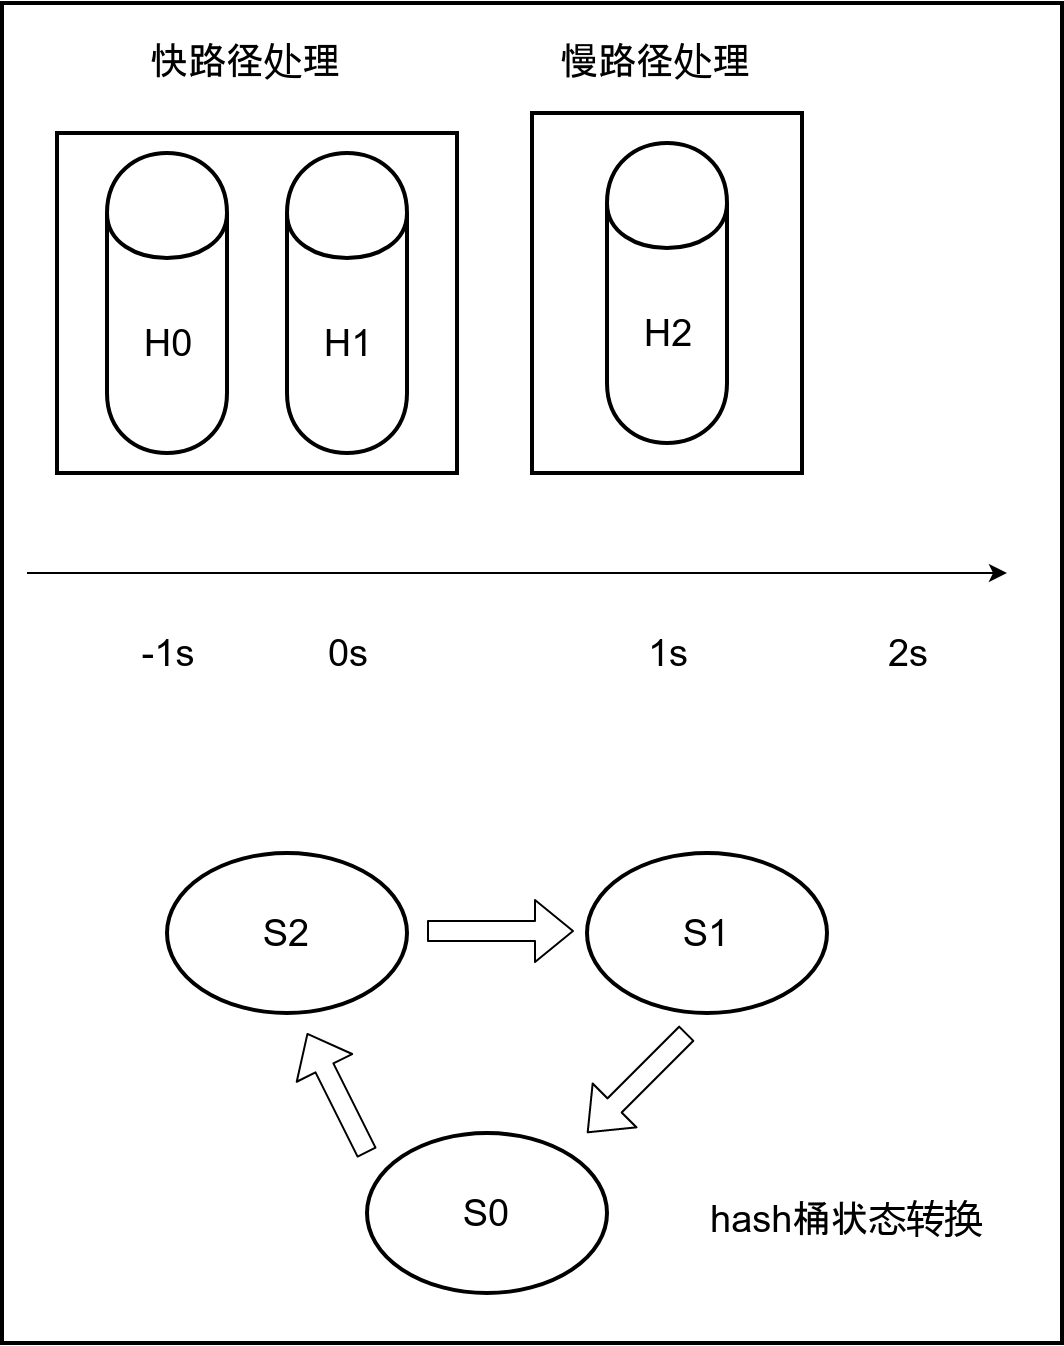
\includegraphics[width=0.8\textwidth]{../img/hash_backet.png}
  \caption{hash backet}
  \label{fig:hash_backet}
\end{figure}


  根据上图\ref{fig:hash_backet}中的状态转换方式, 设计如下两个线程, 分别进行快慢路径的
处理. 将定时器放在了快路径线程中, 通过定时器的触发来推动状态转换. 如果慢路径的
处理时间过久, 将会被\textbf{while(!is\_slow\_over)\{\}}所阻塞, 这不是我们想要看到
的结果, 之后可能会增加统计功能, 用以确定和解决程序的瓶颈.

\begin{lstlisting}[caption=数据结构,frame=tlrb]{Name}
hash_backet* H0, H1, H2;    // 三个hash数据桶
bool is_slow_over = true;   // 标示慢路径是否完成处理
Mutex lock;                 // 互斥锁, 防止快慢路径同时对数据进行修改

\end{lstlisting}

\noindent\begin{minipage}{.55\textwidth}
\begin{lstlisting}[caption=快路径线程,frame=tlrb]{Name}
clock_t start = clock();
while(!stop) {
  p = GetPacket();
  if(H0 found trace) {
    将p添加至H0中;
  } else {
    将p添加至H1中;
  }

  // 超过1s
  while(clock() - start > 1000)
  {
    // spinlock 检查慢路劲处理是否结束
    while(!is_slow_over){}
    TMP = H0;
    H0 = H2;
    H2 = H1;
    H1 = TMP;
    {
        MutexLock;
        is_slow_over = false;
    }
    // 更新clock
    start = clock();
  }
}
\end{lstlisting}
\end{minipage}\hfill
\begin{minipage}{.38\textwidth}
\begin{lstlisting}[caption=慢路径线程,frame=tlrb]{Name}
while(!stop) {
  while(is_slow_over){}
  // 处理慢路径

  {
    MutexLock;
    is_slow_over = true;
  }
}
\end{lstlisting}
\end{minipage}



\section{数据结构}
\label{chap:数据结构}

\textbf{GRE数据包}

\begin{figure}[htbp!]
  \centering
  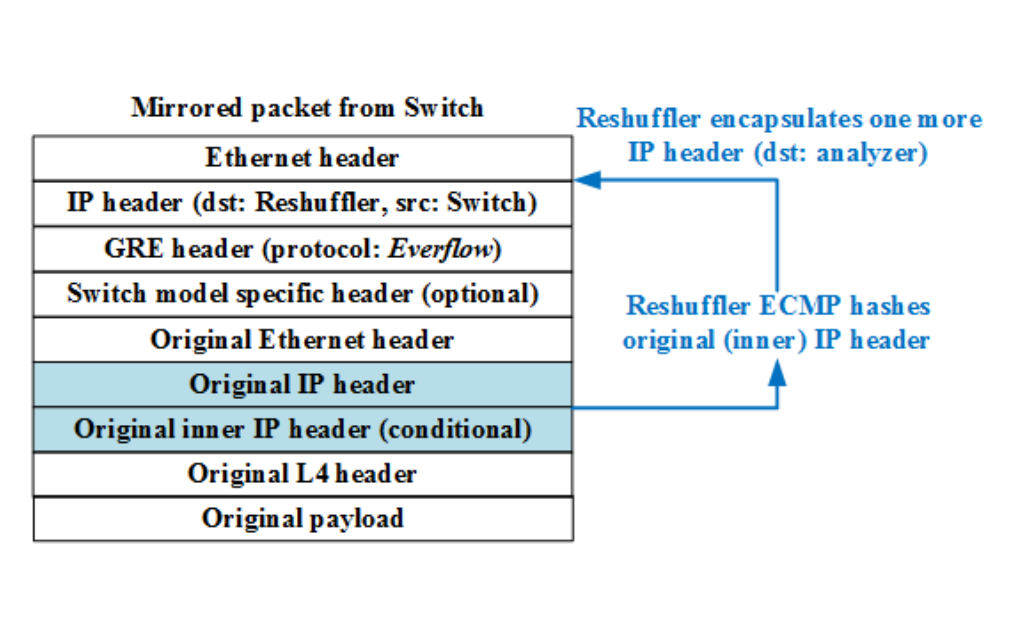
\includegraphics[width=0.6\textwidth]{../img/format_gre.png}
  \caption{GRE packet}
  \label{fig:gre_packet}
\end{figure}

对于到达分析器的数据包来说, 均是使用GRE(Generic Routing Encapsulation)
进行封装, GRE格式见图\ref{fig:gre_packet}.

\textbf{Trace数据}

分析器中存储结构: 基于由于上述分析,
传入任意的分析器中的是一个个单独的数据包, 分析器中, 需要还原整条路径,
但是一条路径上数据包信息是相同的, 所以保存一份即可.
这里是还原后采用的trace路径表示形式. 另外对于每一条trace数据,
还具有一些元数据, 用以表示本trace数据的各种信息.

\begin{lstlisting}

typedef struct{
    struct in_addr ip_src; /**< 32bits 源IP地址   */
    struct in_addr ip_dst; /**< 32bits 目的IP地址 */
    uint16_t ip_id;        /**< 16bits 标识符     */
    uint8_t protocol;      /**< 8bits  协议字段   */
} __attribute__((packed)) IP_PKT_KEY_T;

enum {TRACE_CNT = 5};   /**< 只记录5跳信息 */

/**
 * @brief trace数据结构
 */
typedef struct{
    IP_PKT_KEY_T key;

    uint16_t pkt_size;   /**< 16bits 数据包大小  */

    /**
     * 32bits 收到第一个报文的时间戳: 如果使用秒级的计数单位, 是无法刻画出真实
     * 的数据包的时间情况, 这里的时间戳是毫秒级别的时间戳.
     *
     *  Timestamp记录收到报文的时间,
     *  如果对于某一跳交换机超过1秒还没收到其它的报文, 则视为丢包
     */
    uint32_t timestart;

    struct {
        uint16_t switch_id: 12;
        uint16_t hop_rcvd : 2;
        uint16_t hop_timeshift: 10; /**< 与timestart相减得到的偏移, 也为ms */
    } __attribute__((packed)) hop_info[TRACE_CNT - 1];

    uint16_t hp1_switch_id: 12; /**< 第一跳交换机id          */
    uint16_t hp1_rcvd: 2;       /**< 第一跳交换机收到的报文数  */
    uint16_t used: 1;           /**< 以hash表进行存储,
                                     记录hash表中的当前元素是否被占用. */

    uint16_t is_loop: 1;
    uint16_t is_drop: 1;
    uint16_t is_timeout: 1;
    uint16_t is_probe: 1;

    uint16_t reserved : 5;
} __attribute__((packed)) PKT_TRACE_T;
\end{lstlisting}


除此之外, 分析器中还有计数器, 记录每个规则下的trace数据个数.

在程序中, 需要经过快路径, 慢路径两个处理过程, 由快路径处理结束后,
进入慢路径.

\section{数据库设计}
\label(chap:数据库设计)

存储器中的结构: 使用关系型数据库进行存储.

存储路径的数据表分为三大部分:

\begin{itemize}
    \setlength\itemsep{0.1em}
    \item 第一部分是数据包原始信息, 包括数据包头部以及负载信息.
    \item 第二部分是每一跳的信息, 比如时间戳, 源MAC地址. 每个trace数据跳数不同,
            所以保存 时, 将所有跳的信息结合在一起存储.
    \item 第三部分是元数据信息, 表示这个trace信息是否有环, 是否丢包,
            是否为探针数据.
\end{itemize}


\begin{table}[]
    \centering
    \caption{tbl\_traffic\_data}   % \caption{} 改为 \captionof{table}{}
    \begin{tabular}{llll}   \hline
    Field          & Type          & Comment                   \\ \hline
    id             & int(11)       &                           \\
    s\_ip          & int(11)       & 源IP                       \\
    d\_ip          & int(11)       & 目的IP                      \\
    protocal       & int(11)       & 协议类型                      \\
    generate\_time & timestamp     & 产生时间                      \\
    trace\_data    & varchar(1024) & trace数据信息, 保存为二进制字符串    \\
    fdate          & int(11)       & 存入日期, 如果数据量过大则使用索引 \\
    is\_loop       & int(11)       & 是否有环                      \\
    is\_drop       & int(11)       & 是否丢包                      \\
    is\_probe      & int(11)       & 是否为探针                    \\ \hline
    \end{tabular}
    \label{tbl_traffic_data}
\end{table}

存储计数器的数据表相对简单, 主要记录分析器ID, 计数值以及产生时间.

\begin{table}[]
    \centering
    \caption{tbl\_counter}
    \label{tbl_counter}
    \begin{tabular}{lll} \hline
    Field          & Type          & Comment \\ \hline
    id             & int(11)       &         \\
    counter\_name  & varchar(1024) & 计数器名称   \\
    generate\_time & timestamp     & 数据产生时间  \\
    analyer\_id    & int(11)       & 分析器ID   \\
    cnt            & int(11)       & 计数值     \\
    fdate          & int(11)       & 数据产生日期  \\ \hline
    \end{tabular}
\end{table}
% 主要数据结构及算法 }}}

% {{{ 设计中的一些抉择
\chapter{设计中的一些抉择}
\label{chap:设计中的一些抉择}

\section{技术选型}

此次系统设计, 技术选型主要包括分析器, 存储器, 以及控制器,
上层应用程序的设计.

根据对性能的不同要求, 结合开发进度做以下讨论. 在分析器中,
需要考虑大量的流量 涌来, 必须充分利用系统资源进行数据的接受和处理,
使用偏向底层的C/C++语言, 在控制器中, 只涉及简单的数据库查找与用户交互,
对性能要求不高, 故使用Python, 以实现迅速而 敏捷的开发.

对于本次的系统设计, 分工如下:

\begin{itemize}
\item
  分析器采用C/C++完成
\item
  存储器可能选择MySQL作为存储
\item
  控制器主要通过Python实现, 期间某些静态库的编写使用C/C++完成.
  控制器的API接口采用HTTP协议交互, 最终的展示页面,
  功能配置也将在网页上进行操作, 其中, 图表展示打算使用开源的echarts.
\end{itemize}

\section{路径存储的选择(分析器)}

由于对于某个数据包的整条路径, 我们是需要进行存储的. 但是,
路径存储到数据库后, 我们不打算提供对于数据路径的检索功能. 这样,
可以将所有字段结合在一起放置在数据库中.

对于该字段, 曾经我考虑使用\texttt{Protobuf}与\texttt{JSON}两种.
最终选择了\texttt{JSON}, 主要有 以下两个原因:

\begin{enumerate}
\def\labelenumi{\arabic{enumi}.}
\item
  \texttt{JSON}不只是在存储中用到了,
  在\texttt{Watcher}与控制器交互过程中, 也全部使用了\texttt{JSON} 因此,
  使用\texttt{JSON}能减少项目依赖的类库数量.
\item
  \texttt{Protobuf}在存入数据库时, 需要采用特定的数据结构. 存入取出时,
  对于开发者来说 并不容易使用肉眼调试分析.
\end{enumerate}

鉴于此, 我放弃了内存占用量较小的\texttt{Protobuf},
转而使用易于读取理解的\texttt{JSON}.


\section{有关程序性能的问题(控制器)}

  对于\texttt{CPython}来说, 由于全局中断锁也就是\texttt{GIL}的存在, \texttt{CPython}
无法充分的利用多核. 因此, 编写控制器时, 我选择单线程, 也因此选择了\texttt{Tornado}.

但请知悉所有用户均是在一个线程中进行轮转, 如果某个用户请求时间过久,
将会严重影响其他用户的查询体验.

\section{有关预警方式的选择}

  预警也是本程序应有的功能, 为了开发以及未来其他接入功能的开发, 我采用了\texttt{PushBear}
服务, 用户可以直接扫描二维码关注预警频道. 而后将会收到预警信息. 也可以在任意
时刻取消订阅.

\begin{figure}[htbp]


\centering
\begin{minipage}{0.76\textwidth}

    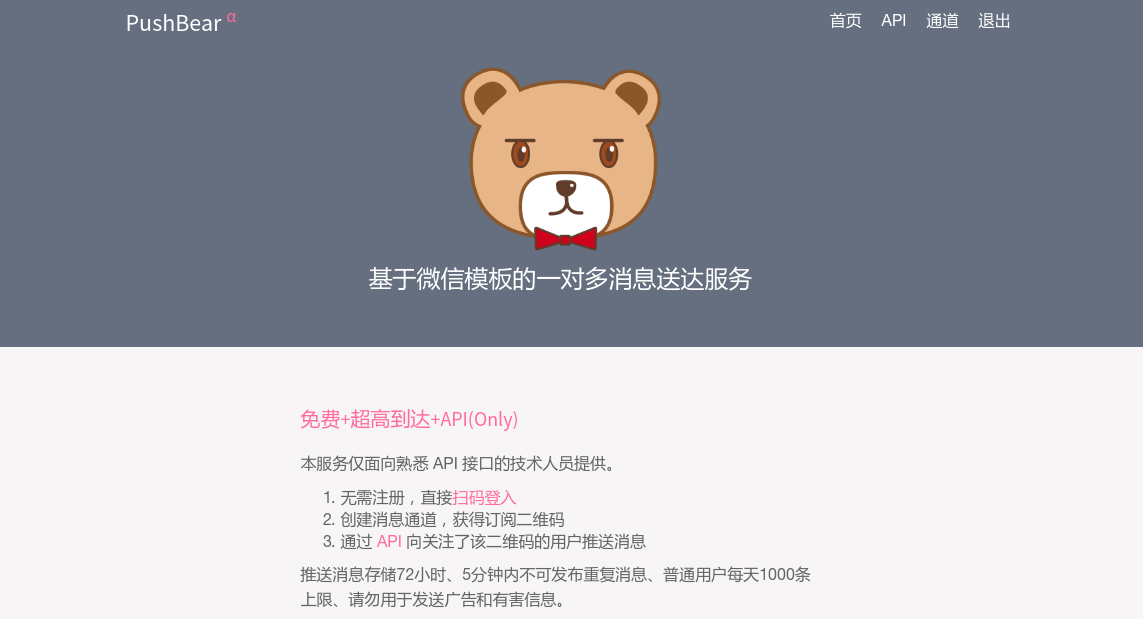
\includegraphics[width=1\textwidth]{../img/pushbear.png}
    \caption{PushBear官网}
    \label{fig:pushbear}

\end{minipage} \hfill
\begin{minipage}{0.22\textwidth}

\centering
    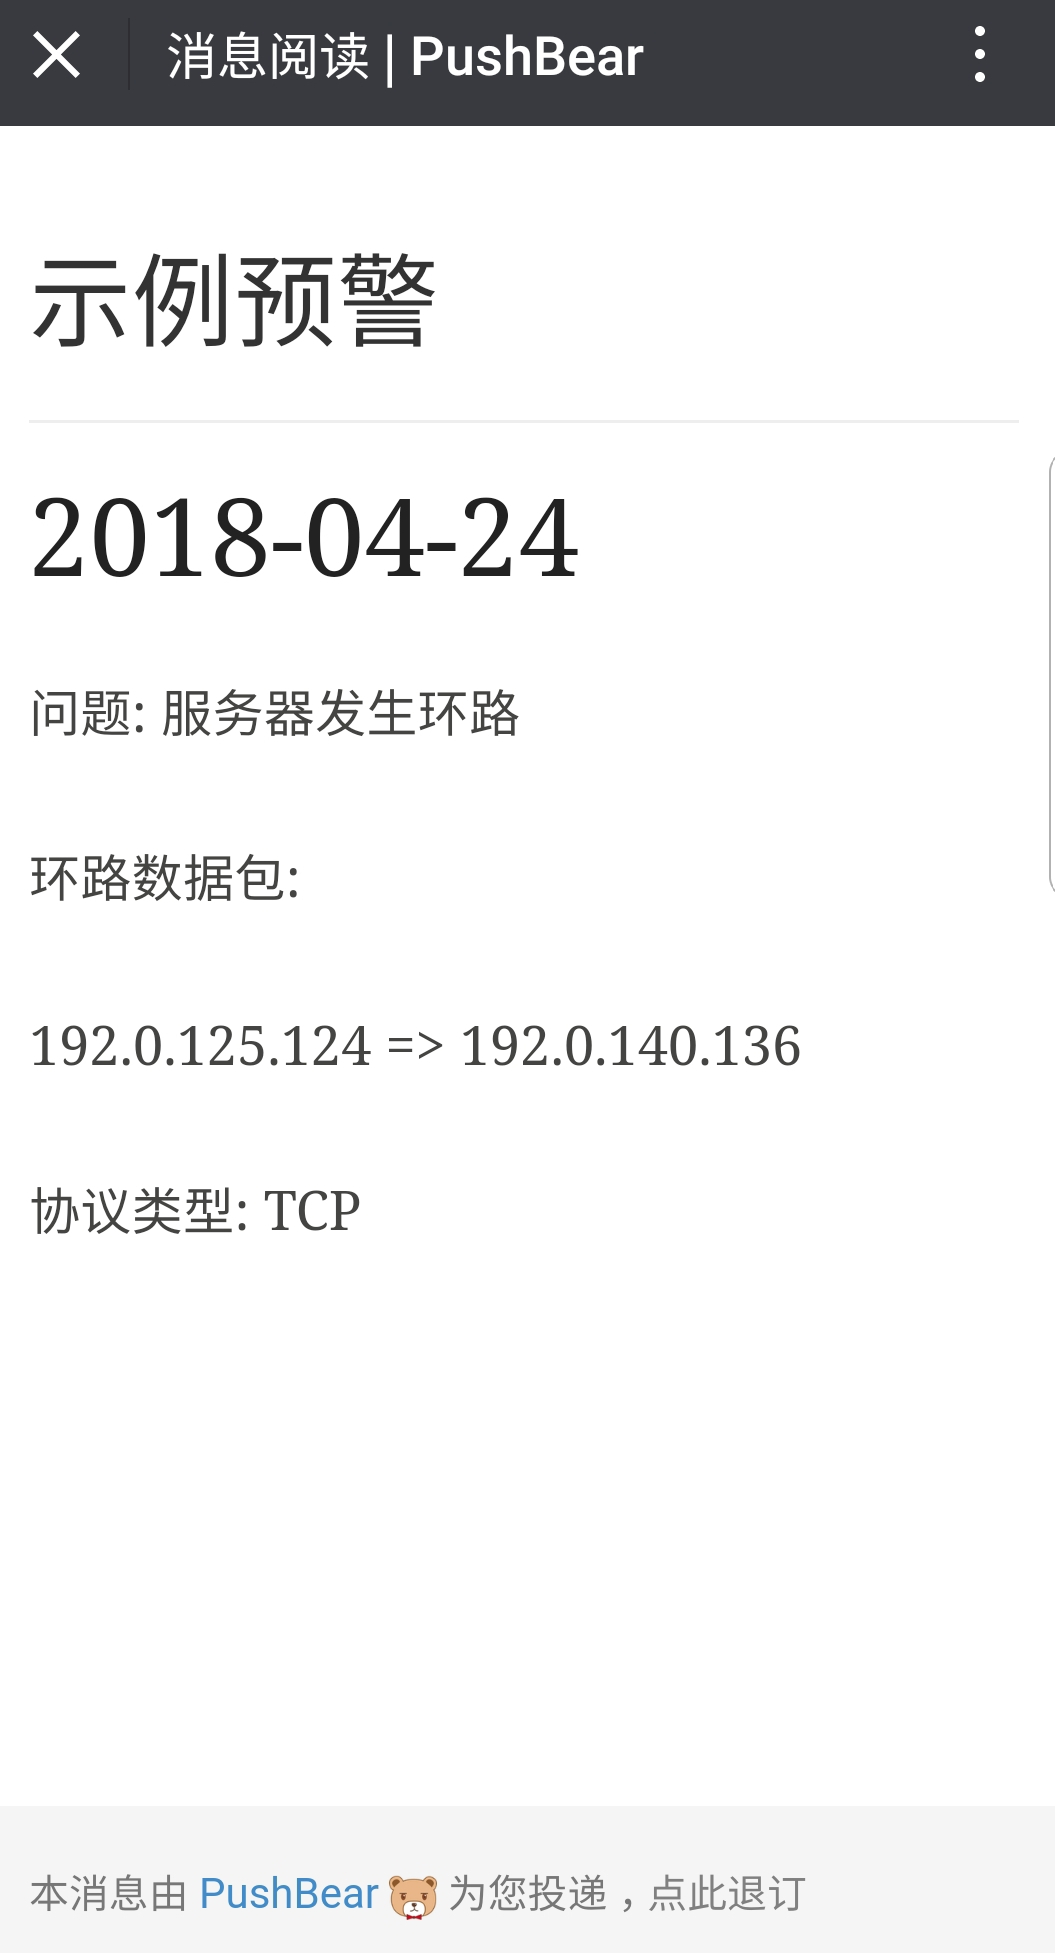
\includegraphics[width=1\textwidth]{../img/push_example.jpg}
    \caption{推送样例}
    \label{fig:push_example}
\end{minipage}

\end{figure}

如图\ref{fig:pushbear}为官网, 右侧\ref{fig:push_example}为推送样例.

%  https://pushbear.ftqq.com/admin/#/
%  设计中的一些抉择  }}}

%  {{{ 程序部署
\chapter{程序部署}

  本次的程序设计主要分为三个部分, 分析器, 存储器以及控制器, 展示页面由控制器
负责加载. 承接上文分析器控制接口设计\ref{sec:分析器, 控制器接口设计}, 分析器, 
控制器, 与存储器之间是不存在耦合的, 均可进行单独的部署.

  它们之间唯一需要的只有TCP连接. 另外, 有关Redis服务器, 我选择与存储器放置在一台
服务器上. 最主要的原因就是Redis以及MySQL的存在, 就是为了连接分析器与控制器,
放置在一台服务器上符合它们的作用.

  另外, 分析器可以在多台PC进行部署, 这是由于一条路径上的所有数据包都会根据hash操作
分配至同一个分析器中. 可以利用这一特性, 进行横向扩展来提高系统的吞吐量.

  有关详细的部署操作, 在代码的文档中均有记录, 在此不进行赘述.
% 程序部署 }}}

\chapter{性能测试情况}

  程序中, 实现的功能有下面这些:

\begin{itemize}
    \item 对分析器: 包括有网卡数据读取, 快慢路径处理数据, 有问题的Trace数据入库,
计数器报告, 报警信息发送.
    \item 对存储器: 读写有问题的Trace, 读写计数值.
    \item 对控制器: 分析器的初始化, 提供数据访问接口, 添加删除规则, 探针的发送.
\end{itemize}

  对于存储器来说, 只负责存储异常的数据包信息以及提供访问能力, 建立合适的索引之后,
数据库可以保持较好的性能, 而控制器只负责控制分析器与提供接口, 数据量并不大.
其中性能存在瓶颈部分的主要在于分析器中,

\section{评测环境}

服务器配置如下:

\begin{table}[]
    \centering
    \caption{服务器配置}
    \label{server_config}
    \begin{tabular}{ll} \hline
    Field    & Type          \\ \hline
    CPU:     & Intel(R) Xeon(R) CPU E5-2690 v4 @ 2.60GHz \\
    内存:      & 32G                                       \\
    监听的网卡为lo & 采用tcpreplay指定测试数据以及发送速率. \\ \hline
    \end{tabular}
\end{table}


\section{评测过程}

\begin{itemize}
    \item 首先启动分析器程序
    \item tcpreplay进行大量的数据包发送, 评测时的输入8000pps(packets per second).
    \item 程序的内存占用率一直上升, 我便在一段时间后将发包程序关闭.
        图\ref{fig:queue_pic} 中的最高点即关闭发包程序的时刻, 此时队列中
        不再增加数据的状态, 图\ref{fig:process_pic}中为线程的处理情况.
\end{itemize}

\section{结果概述}

 下面两张图对应的均为日志记录为\texttt{INFO}的情况. 对于日志记录为\texttt{DEBUG}
的情况, 生成的日志过于庞大, IO占了很大一部分性能, 大概要比INFO时的性能损失4-5倍,
同时, 内存也未能充分利用.

\begin{figure}[htbp!]
  \centering
  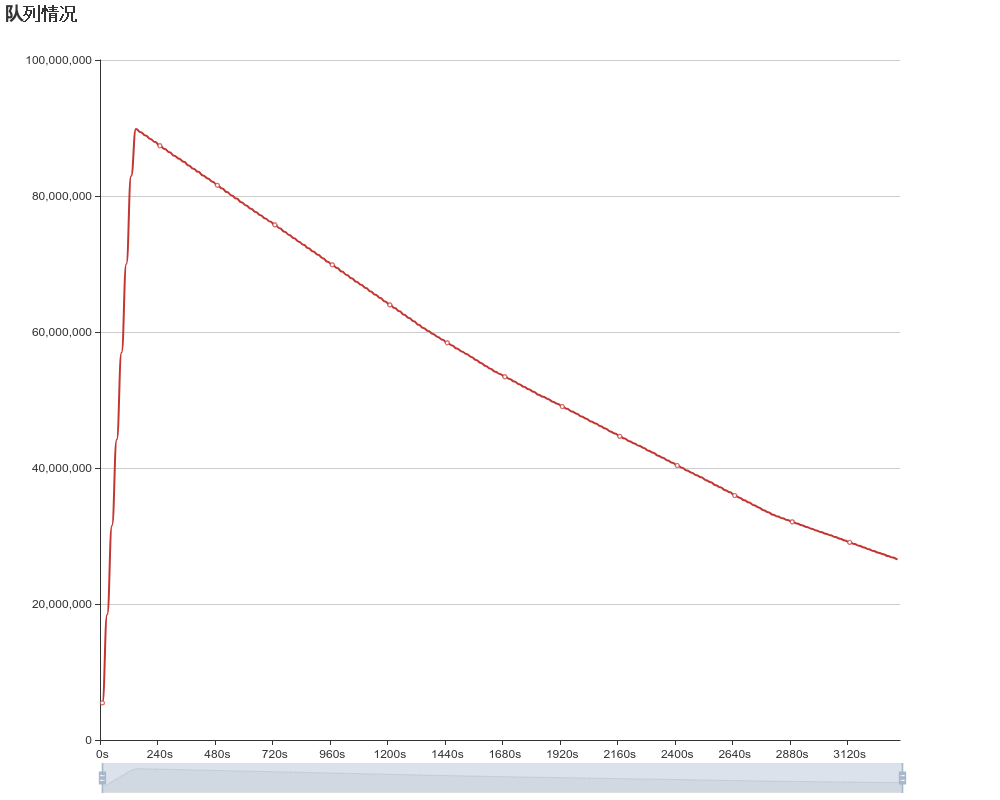
\includegraphics[width=0.8\textwidth]{../img/队列情况-info.png}
  \caption{队列中数据变化}
  \label{fig:queue_pic}
\end{figure}

\begin{figure}[htbp!]
  \centering
  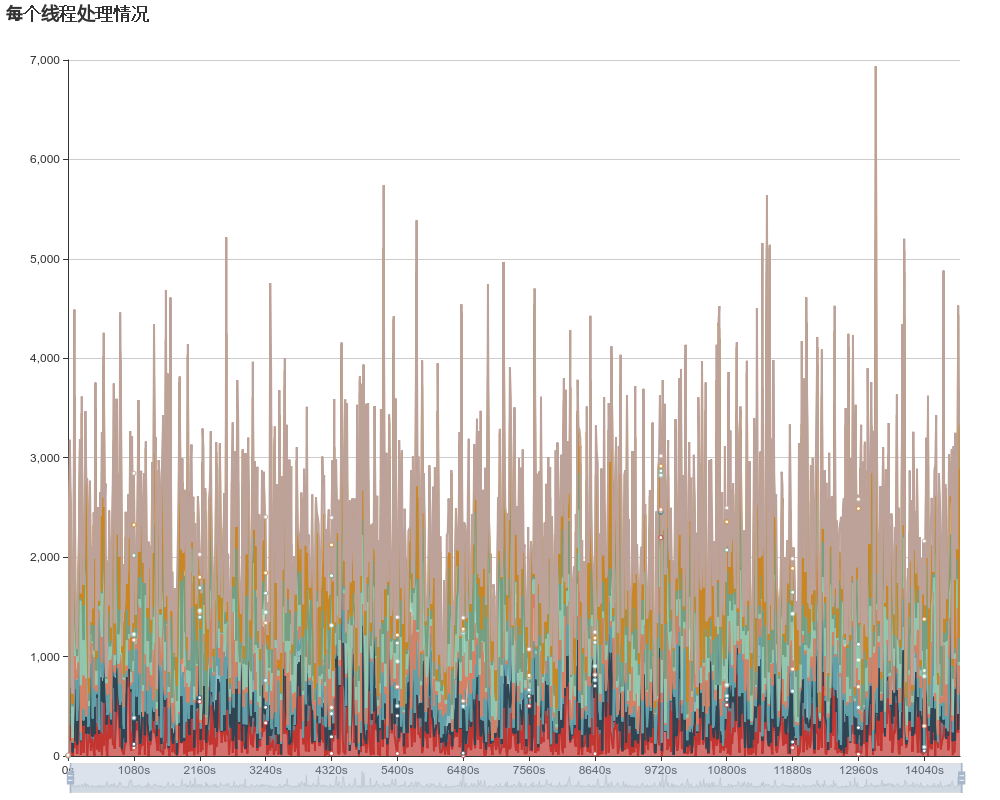
\includegraphics[width=0.8\textwidth]{../img/每个线程处理情况-info.png}
  \caption{各个线程处理情况}
  \label{fig:process_pic}
\end{figure}

其中, 我取了队列变化过程中的两个点(160s, 89376014), (2900s, 31841057), 计算得到
$$ \frac{89376014 - 31841057}{2900 - 160} = 20998 pps $$
20000多的pps, 是比较正常的吞吐量了.


具体的评测请查看\texttt{analyzer/README.md}中的性能评测部分, 我介绍了相对详细的
评测过程以及结果分析.

% \chapter{扩展}

